\documentclass[paper=a4, fontsize=11pt]{scrartcl}
\usepackage{enumerate}
\usepackage{amsmath}
\usepackage{tikz}
\newcommand{\parens}[1]{ \left( #1 \right) }
\begin{document}
  \begin{center}
    STAT 221: Problem Set 2 \\
    Kevin Eskici and Willy Xiao \\
    Due: Oct 7, 2014
  \end{center}
  \begin{enumerate}[\text{Task }1:]
    \item Examine the Posterior \\

      Posterior is: $f(\mu, \sigma^2, \log{\vec{\theta}} | Y)$
      \begin{align*}
        f(\mu, \sigma^2, \log{\vec{\theta}} | Y) &\propto f(Y|\log{\vec{\theta}}) * f(\log{\vec{\theta}}|\mu, \sigma^2) * f(\mu, \sigma^2) \\
        &\propto \prod_{j=1}^{J}{
          \left[ \parens{
            \prod_{i=1}^N{
              e^{-w_je^{\log{\theta_j}}}\parens{w_je^{\log{\theta_j}}}^{Y_{ji}}
            }}
            * \frac{1}{\sigma}e^{
                                  \frac{-(\log{\theta_j}-\mu)^2}{2\sigma^2}
                                }
            * \frac{1}{\sigma^2}
          \right]
        }
      \end{align*}
      The Posterior of $\log{\theta}$ conditional on all the other parameters is the same as the previous equation, except we can drop the prior on $\mu$ and $\sigma^2$ because they're given:
      \begin{align*}
        f(\log{\theta} | Y, \mu, \sigma^2)
          &\propto \prod_{j=1}^{J}{
            \left[ \parens{
              \prod_{i=1}^N{
                e^{-w_je^{\log{\theta_j}}}\parens{w_je^{\log{\theta_j}}}^{Y_{ji}}
              }}
              * \frac{1}{\sigma}e^{
                                    \frac{-(\log{\theta_j}-\mu)^2}{2\sigma^2}
                                  }
            \right]
          }
      \end{align*}
      To check the shape of the function, we can look at the second derivative of the log-posterior:
      \begin{align*}
        \text{ Let } \log{p} &= \log{f(\log{\theta} | Y, \mu, \sigma^2)} \\
          &= \sum_{j = 1}^J{
            \parens{
              \sum_{i = 1}^N{ \parens{
                -w_je^{ \log{ \theta_j }} + Y_{ji}*\parens{ \log{w_j} + \log{e^{\log{\theta_j}}} }
              }}
              - \log{\sigma}
              - \frac{ \parens{ \log{\theta_j} - \mu}^2}{2\sigma^2}
            }
          } \\
        \frac{\partial{\log{p}}}{\partial{\log{\theta_j}}}
          &= \sum_{j=1}^J{
            \parens{
              \sum_{i=1}^N{ \parens{
                -w_je^{\log{\theta_j}} + Y_{ji}\log{\theta_j}
              }}
              - \frac{\log{\theta_j} - \mu}{\sigma^2}
            }
          } \\
        \frac{\partial^2{\log{p}}}{\partial{\log{\theta_j}}^2}
          &= \sum_{j=1}^J{
            \parens{
              \sum_{i=1}^N{ \parens{
                -w_je^{\log{\theta_j}} + Y_{ji}
              }}
              - \frac{1}{\sigma^2}
            }
          }
      \end{align*}
      Because the second derivative of the log-posterior is monotonically decreasing with respect to $\log{\vec{\theta}}$, that means our function is unimodal (ie there's a single peak).
    \item Write functions to simulate data from the model \\

      Check keskici\textunderscore wxiao\textunderscore ps2\textunderscore functions.R
    \item Evaluate coverage for a simple case \\

      First: Estimate the amount of simulations we can do:
        \begin{enumerate}
          \item The time it took to run one simulation on my Macbook Air was roughly 23 seconds. Accounting for startup costs (copying to multiple machines, however Odyssey decides to manage nodes etc.,), we roughly said that each MCMC simulation would take 25 seconds.
          \item Calculating, we have
            \begin{align*}
              (60 \text{ seconds}) \times (60 \text{ minutes}) \times (12 \text{ nodes}) = 43200 \text{ seconds of runtime.}
            \end{align*}
              Then
            \begin{align*}
              \frac{43200}{(4 \text{ parameters})} / (25 \text{ seconds per simulation}) = 432 \text{ simulations per parameter.}
            \end{align*}

          We ultimately decided to go with $360$ simulations per parameter to guarantee that we don't go over the hard one-hour time limit. Also $360$ is a number that is divisible by $12$ and easily modeled on our local machines to test (e.g. running 36 simulations rather than 360), which makes writing the .slurm job a little bit easier.
        \end{enumerate}


      Second: Decide how many theta's to draw and how many Y's to draw: \\
        Ultimately we weren't sure how best to do this. The example on the pset had more theta draws than Y draws, so we decided to do the same.
        \begin{align*}
          \text{ theta.draws } &= 30 \\
          \text{ Y.draws } &= 12
        \end{align*}

      Third: RUN! :) \\

      Unfortunately, the timing was wildly off. It didn't take into account that we had to calculate the coverage after each theta draw which means we had to recalculate how many times simulations we could do! We tried 
      $12 \times 15$ (ie half of what it was before, and it still went too long), $12 \times 12$ was close. Ultimately we ran it for:
      \begin{align*}
        \text{ theta.draws } &= 9 \\
        \text{ Y.draws} &= 15 \\
      \end{align*}

    \item Evaluate coverage with exposure weights \\

      We ran the same simulation as Task 3, except we added in the exposure weights. Results discussion below, code in relevant file.
    \item Evaluate coverage with model misspecifcation: \\
      We ran the same simulation as Task 4, substituting in rASL instead of rnorm as our function to generate $\log{\theta_j}$. For running the MCMC simulation, we left the parameters mu and sigmasq to be their defaults $0$ and $1$ respectively.
	\item Interpretation of results:\\
	We noticed that the coverage percentages in task 3 seemed to peak around the true value of $\mu$ for both the 68\% and 95\% confidence intervals. Additionally, we see in figures 1 and 2 that the coverage percentages were far lower than 65/95 for low values of theta than they are in figures 3 and 4 (though in figures 1 and 2 the coverage percentages rapidly increase as we approach the true parameter value before having a slgiht dip). From this we can infer that when we have higher values of $\mu$, the frequentist coverage properties hold better. This can be explained by the prior proportionally having less weight in the posterior when our values of $\mu$ are higher. It is easiest to see this effect by comparing figures 3 and 4 because they were generated with the same values of $\sigma^2$ with different $\mu$s. It is also interesting to note that while there was an increase in $\mu$ in figure 2 compared to figure 1, the increase in variance seems to have partially offset it leaving the 68\% coverages pretty similar. In the 95\% CI case the increased variance seemed to have less of an impact and the coverages were better for low values of $log(\theta_{j})$.\\
	In task 4 we added exposure weights to the mix. Comparing the figures for task 4 (figures 5,6,7, and 8) to their corresponding figures for task 3(figures 1,2,3, and 4 respectively), we see that the addition of exposure weights to the model made the coverage peaks at the true values of $\mu$ more pronounced. Again we saw that this peak coverage was not much higher than the rest of the curve for cases where our $\mu$s were higher (comparing figures 5 and 6 to figures 7 and 8). We also see that the coverage curves for the $log(w_j)$ are almost horizontal at 68/95, and are flatter for the cases with higher $\mu$s as seen in figures 7 and 8 as opposed to figures 5 and 6 where they seem to curve a bit before converging to a line at 68/95 after a certain threshold.\\
	In task 5  we evaluated coverage for a misspecified model. Given this, it is no surprise that the coverage rates were the furthest from 68/95 for this model. Comparing figures 10 and 11 we see that added the $.7X$ term instead of subtracting it gives us much better coverage, which again seems like a result of there being a higher mean (and the model isn't AS off (though it is still misspecified) in that case). Interestingly it seems the weights have a bit more of an effect for the parameters shown in figure 11 than they do in figure 10. Comparing figures 9 and 12 we also see that increasing our error term (and thus also the variance) doesn't have as much of an effect on coverage in our misspecified model, likely because without the exponential term our prior still has a large weight in both cases.\\
	Overall we see that the more weight our prior is given in our posterior distribution relative to the liklihood, the less frequentist coverage properties hold.
  \end{enumerate}
\clearpage
Appendix: \\
\begin{figure}[h!]
  \caption{Task 3 coverage plots for $log(\theta_{j}$)'s : $\mu = 1.6$, $\sigma^2 = 0.7^2$}
  \centering
	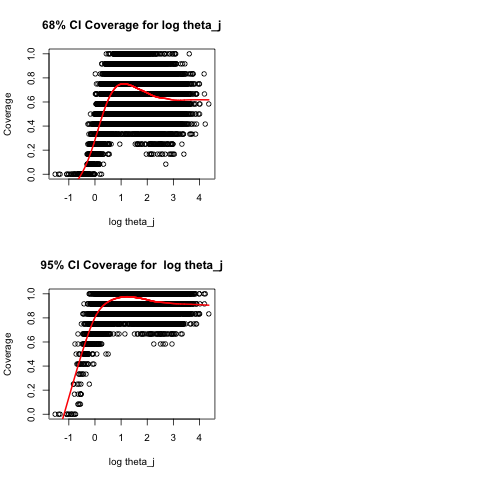
\includegraphics[scale=1, trim = 0 0 200 0]{keskici_wxiao_ps2_task3_plot1.png}
\end{figure}

\begin{figure}[h!]
  \caption{Task 3 coverage plots for $log(\theta_{j}$)'s : $\mu = 2.5$, $\sigma^2 = 1.3^2$}
  \centering
	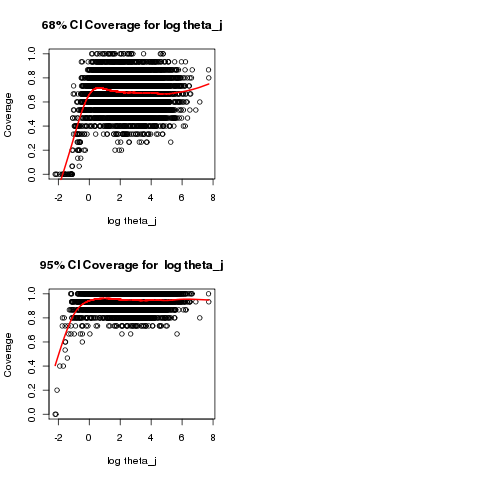
\includegraphics[scale=1, trim = 0 0 200 0]{keskici_wxiao_ps2_task3_plot2.png}
\end{figure}

\begin{figure}[h!]
  \caption{Task 3 coverage plots for $log(\theta_{j}$)'s : $\mu = 5.2$, $\sigma^2 = 1.3^2$}
  \centering
	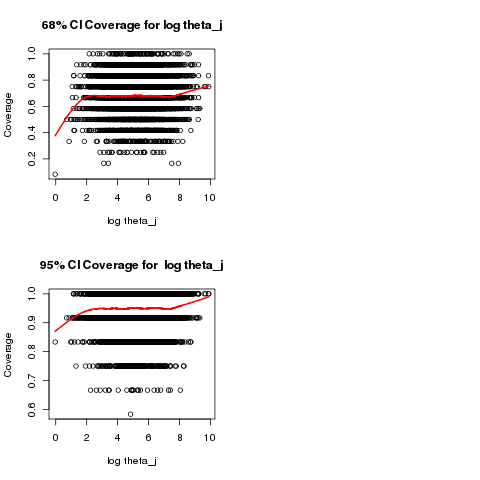
\includegraphics[scale=1, trim = 0 0 200 0]{keskici_wxiao_ps2_task3_plot3.png}
\end{figure}

\begin{figure}[h!]
  \caption{Task 3 coverage plots for $log(\theta_{j}$)'s : $\mu = 4.9$, $\sigma^2 = 1.6^2$}
  \centering
	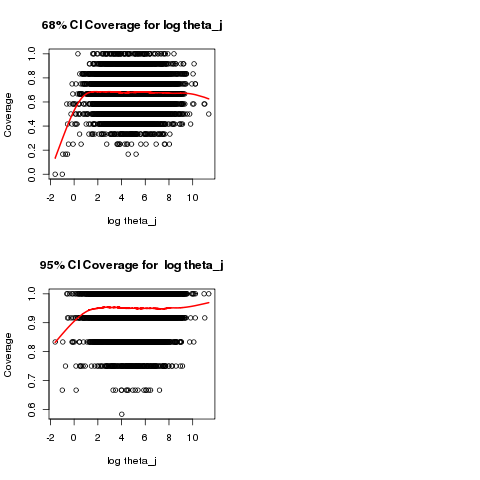
\includegraphics[scale=1, trim = 0 0 200 0]{keskici_wxiao_ps2_task3_plot4.png}
\end{figure}

%%%%%%%%%%%%%%%%%%%%%%%%%%%%%%%%%%%%%%%%%%%%%%%%%%%%%%%%%%%
\begin{figure}[h!]
  \caption{Task 4 coverage plots for $\mu = 1.6$, $\sigma^2 = 0.7^2$}
  \centering
	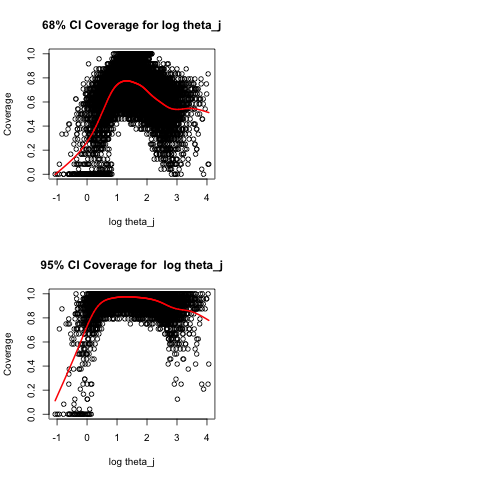
\includegraphics[scale=1, trim = 80 0 150 0]{keskici_wxiao_ps2_task4_plot1.png}
		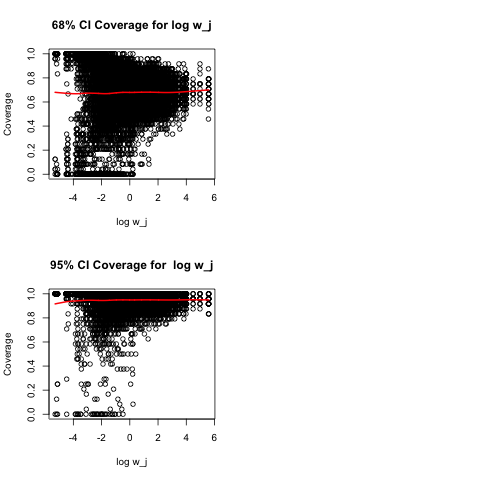
\includegraphics[scale=1, trim = 100 0 300 0]{keskici_wxiao_ps2_task4_plot2.png}
\end{figure}

\begin{figure}[h!]
  \caption{Task 4 coverage plots for $\mu = 2.5$, $\sigma^2 = 1.3^2$}
  \centering
	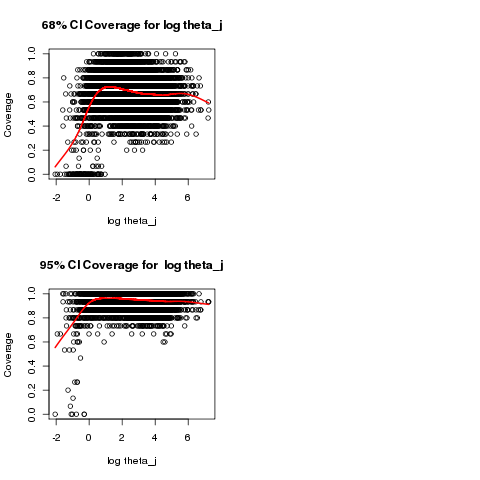
\includegraphics[scale=1, trim = 80 0 150 0]{keskici_wxiao_ps2_task4_plot3.png}
		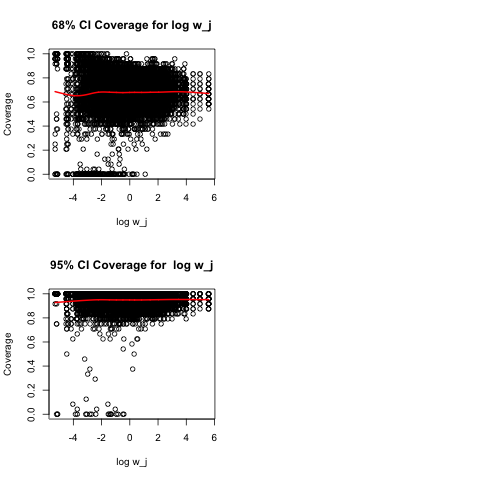
\includegraphics[scale=1, trim = 100 0 300 0]{keskici_wxiao_ps2_task4_plot4.png}
\end{figure}


\begin{figure}[h!]
  \caption{Task 4 coverage plots for $\mu = 5.2$, $\sigma^2 = 1.3^2$}
  \centering
	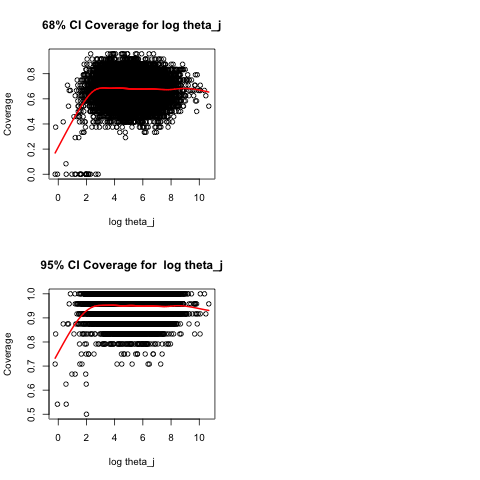
\includegraphics[scale=1, trim = 80 0 150 0]{keskici_wxiao_ps2_task4_plot5.png}
		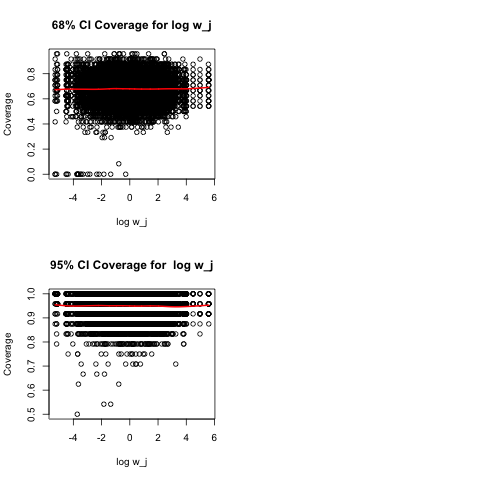
\includegraphics[scale=1, trim = 100 0 300 0]{keskici_wxiao_ps2_task4_plot6.png}
\end{figure}

\begin{figure}[h!]
  \caption{Task 4 coverage plots for $\mu = 4.9$, $\sigma^2 = 1.6^2$}
  \centering
	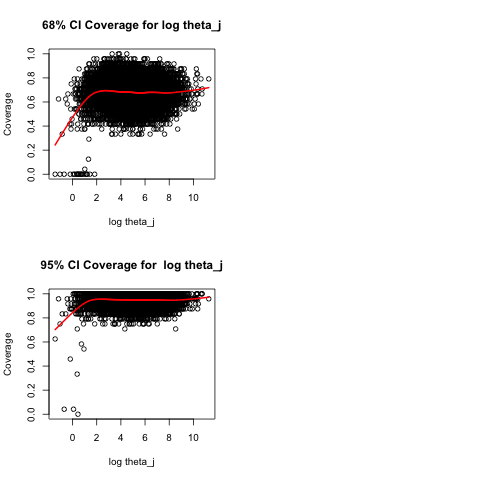
\includegraphics[scale=1, trim = 80 0 150 0]{keskici_wxiao_ps2_task4_plot7.png}
		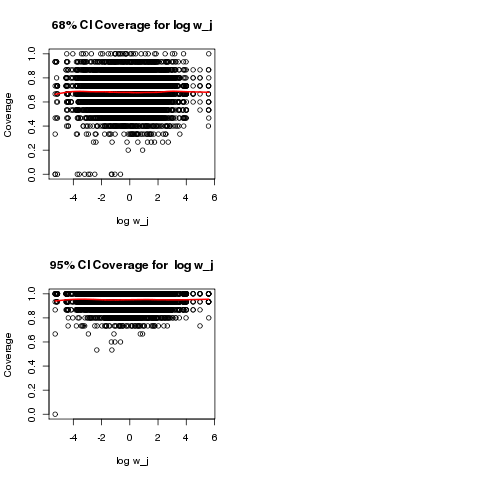
\includegraphics[scale=1, trim = 100 0 300 0]{keskici_wxiao_ps2_task4_plot8.png}
\end{figure}


%%%%%%%%%%%%%%%%%%%%%%%%%%%%%%%%%%%%%%%%%%%%%%%%%%%%%%%%%%
\begin{figure}[h!]
  \caption{Task 5 coverage plots for $log(\theta_{j}$)'s : $x_0 = 1.6$, $m = 0, b = 1.3$}
  \centering
	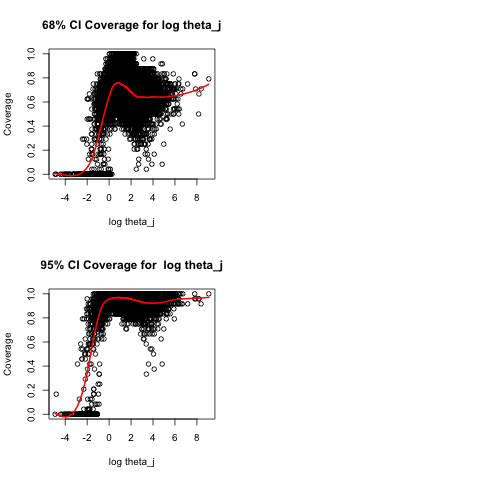
\includegraphics[scale=1, trim = 80 0 150 0]{keskici_wxiao_ps2_task5_plot1.png}
		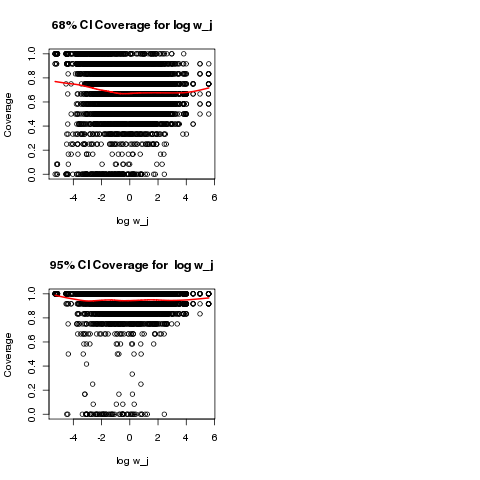
\includegraphics[scale=1, trim = 100 0 300 0]{keskici_wxiao_ps2_task5_plot2.png}
\end{figure}


\begin{figure}[h!]
  \caption{Task 5 coverage plots for $log(\theta_{j}$)'s : $x_0 = 1.6$, $m = -0.7, b = 1.3$}
  \centering
	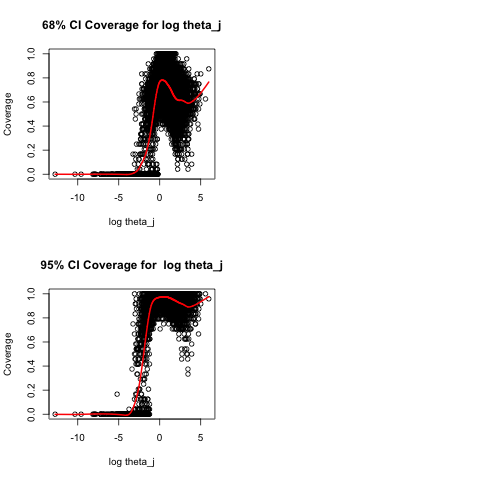
\includegraphics[scale=1, trim = 80 0 150 0]{keskici_wxiao_ps2_task5_plot3.png}
		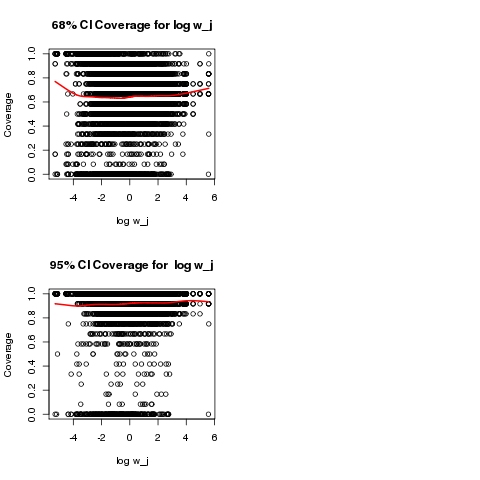
\includegraphics[scale=1, trim = 100 0 300 0]{keskici_wxiao_ps2_task5_plot4.png}
\end{figure}


\begin{figure}[h!]
  \caption{Task 5 coverage plots for $log(\theta_{j}$)'s : $x_0 = 1.6$, $m = -.7, b = 1.3$}
  \centering
	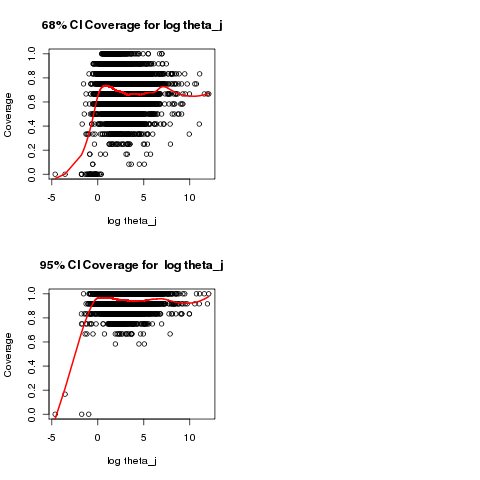
\includegraphics[scale=1, trim = 80 0 150 0]{keskici_wxiao_ps2_task5_plot5.png}
		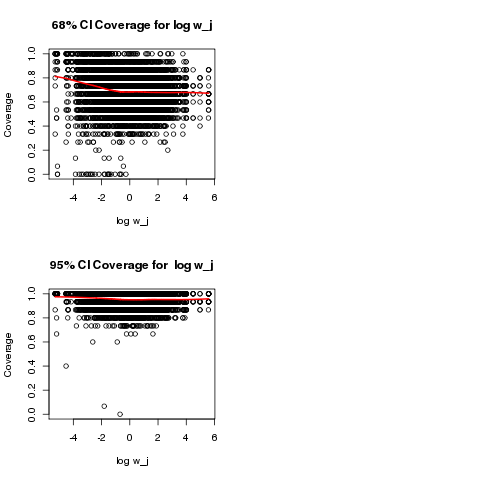
\includegraphics[scale=1, trim = 100 0 300 0]{keskici_wxiao_ps2_task5_plot6.png}
\end{figure}

\begin{figure}[h!]
  \caption{Task 5 coverage plots for $x_0 = 1.6$, $m = 0, b = 2.6$}
  \centering
	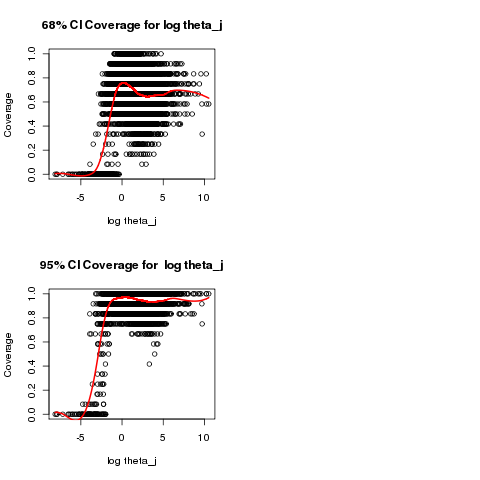
\includegraphics[scale=1, trim = 80 0 150 0]{keskici_wxiao_ps2_task5_plot7.png}
		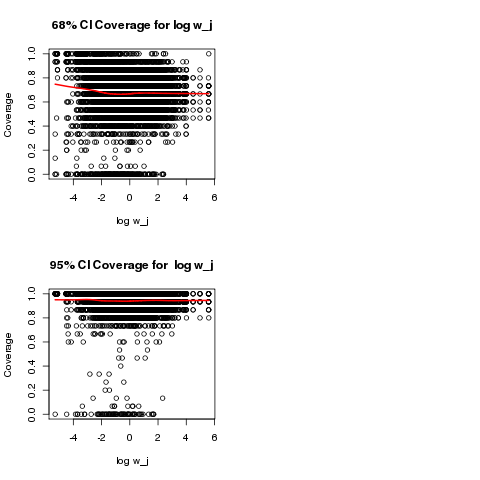
\includegraphics[scale=1, trim = 100 0 300 0]{keskici_wxiao_ps2_task5_plot8.png}

\end{figure}







\end{document}
